%! TEX root = 'main.tex'
\section{Finding Kernel TOCTOU Bugs}
\label{sec:experiment}

%\hb{you need to rewrite this part, I did not get what you want to tell reader. You have to summarize what you will talk in this paragraph first, then goes with the logic, what did you find, how, what are the challenges and how do you solve it smartly }

%One side-project is to find TOCTOU bugs, which is also essential to expose this type of vulnerability.  Previous work such as~\cite{jurczyk2013identifying}~\cite{bochspwnreloaded} utilize a full software emulated virtual machine Bochs~\cite{lawton2003bochs}. It parses and executes each instruction without hardware virtualization assistant or dynamic binary translation.  It is straight forward to instrument the operating system kernel, and it discovers many vulnerabilities of this type~\cite{jurczyk2013identifying}~\cite{bochspwnreloaded}. However, due to the nature of full software emulation, the virtual machine runs extremely slow. Therefore it is not easy to make a comprehensive test, especially with GUI programs, because it needs a prompt response.

%As previously discussed, the SMAP feather is an ideal way of monitoring kernel-to-user-memory behavior. The goal is to check if the same address is being read twice by one system call. However, with the mechanism previously described, once the system protects a user-mode page by setting it to the kernel-mode, the system will not raise the SMAP exception again, which will miss the subsequent kernel accesses. Therefore, instead of protecting a page, we only want to record the information and let the system continue. Unfortunately, we tried different methods to cancel a SMAP exception, and setting the faulting page to kernel-mode is the only way that satisfies the CPU so far. Hence we want to set the protected page back to the user-mode as soon as possible not to lose track of the kernel. 


This section presents our fuzzing tool for kernel-level TOCTOU vulnerability and the result we obtained on the Windows system, especially double-fetch bugs from the Win32k graphical subsystem.


Kernel-level TOCTOU vulnerabilities are subtle. The double-fetch bugs are not intuitive to be aware of by programmers. They are not apparent errors such as buffer overflow that the compiler-based method (cite) can detect. It is even harder to find than the use-after-free vulnerability that code emulation or run-time checks can expose (cite). As described in \autoref{sec:background}, the exploit needs to win the race with the kernel in high speed, and by chance that it can trigger the vulnerability. From previous research works and vulnerabilities' publicly available information, the cause of kernel-level TOCTOU vulnerability is either due to historical reasons that a kernel module is highly coupled with user libraries or because of floppy coding style. However, this vulnerability has a solid memory access pattern, namely, two reads from kernel to userspace. It is not convenient to observe such a pattern either from user programs or the kernel. The most intuitive way is to use a virtual machine. Previous work such as~\cite{jurczyk2013identifying}~\cite{bochspwnreloaded} utilize a full software emulated virtual machine Bochs~\cite{lawton2003bochs}, which parses and executes each instruction without hardware virtualization assistant or dynamic binary translation.  It is straight forward to instrument the operating system kernel, and it discovers many double-fetch vulnerabilities~\cite{jurczyk2013identifying}~\cite{bochspwnreloaded}. However, due to the nature of full software emulation, the virtual machine runs extremely slow. Therefore it is not easy to make a comprehensive test, especially with GUI programs, because GUI needs a prompt response.

As previously described in \autoref{sec:background}, the SMAP feature is an ideal way of monitoring kernel-to-user-memory behavior. The goal is to check if the same address is being read twice by one system call. 

However, the difficulty lies in recovering the system from a fatal \texttt{SMAP} exception.  Because of its original intention, the operating system should crash when it receives such an exception. We tried different methods to cancel a SMAP exception, such as disabling it at \texttt{CR4.SMAP} or temporarily disable it through setting \texttt{EFLAGS.AC}. None of them works.  Fortunately, setting the faulting page to kernel-mode is one way to satisfy the processor so far. Subsequently, we want to set the page back to user-mode as soon as possible not to lose track of the kernel.

\textbf{\textit{Single Step Trap.}} It is the soonest way to get back the control. Through setting the trap flag (TF) in the EFLAGS register, the processor will stop at every instruction. We want to stop at the next instruction that follows the one that triggers the SMAP exception, set back the protected page to user-mode, and continue the kernel. The processor automatically sets the resume flag (RF) in the EFLAGS image on the stack before entry into any fault handler so that the handler will not be interrupted on every instruction. Also, the IRET instruction at the end of the handler should set the RF in the EFLAGS register, so the processor will not generate another trap at the same address. Since we have a hypervisor, the single-step trap triggers a VM exit as a non-maskable interrupt. In the event handler, we clear the TF and set the RF in the guest EFLAGS. Then the hypervisor resumes the guest virtual machine.

\textbf{\textit{Breakpoint}} Nevertheless, the single-step trap still comes in. We decide to write a software breakpoint directly on the first byte of the next instruction. After handling the user-mode page in the SMAP exception handler, we parse the current instruction to get its length. Then we temporarily disable the write protection of the kernel through set CR4.WP and we next write a byte 0xcc to the beginning of the next byte. After that, we record the information of this access and let the kernel continue. When the hypervisor gets the debug trap, we replace the missing byte, release the protected page, and then resume the virtual machine to re-run the faulting instruction. We observe that when the trap happens, in the hypervisor event handler's context, the CR3 register always has the page table base of the SYSTEM process. We need to change it to the target process and then write the missing byte to the right memory space.

\textbf{\textit{Results.}} 
We found a few double fetch bug candidates, and~\autoref{table:doubleread} in~\autoref{sec:evaluation} gives a glimpse of the problem. This method has an advantage over the binary static analysis. Different code segments may use different addressing modes with different bases to access a user-mode address.  It is not obvious to spot if the code segments are slightly apart. For example, in~\autoref{fig:doublefetch}, it needs to trace both ECX and EDX registers and, in some cases, need to get user input to calculate the address. With our solution, it is easy to spot the address after computation at run time.

\begin{figure}[th]
  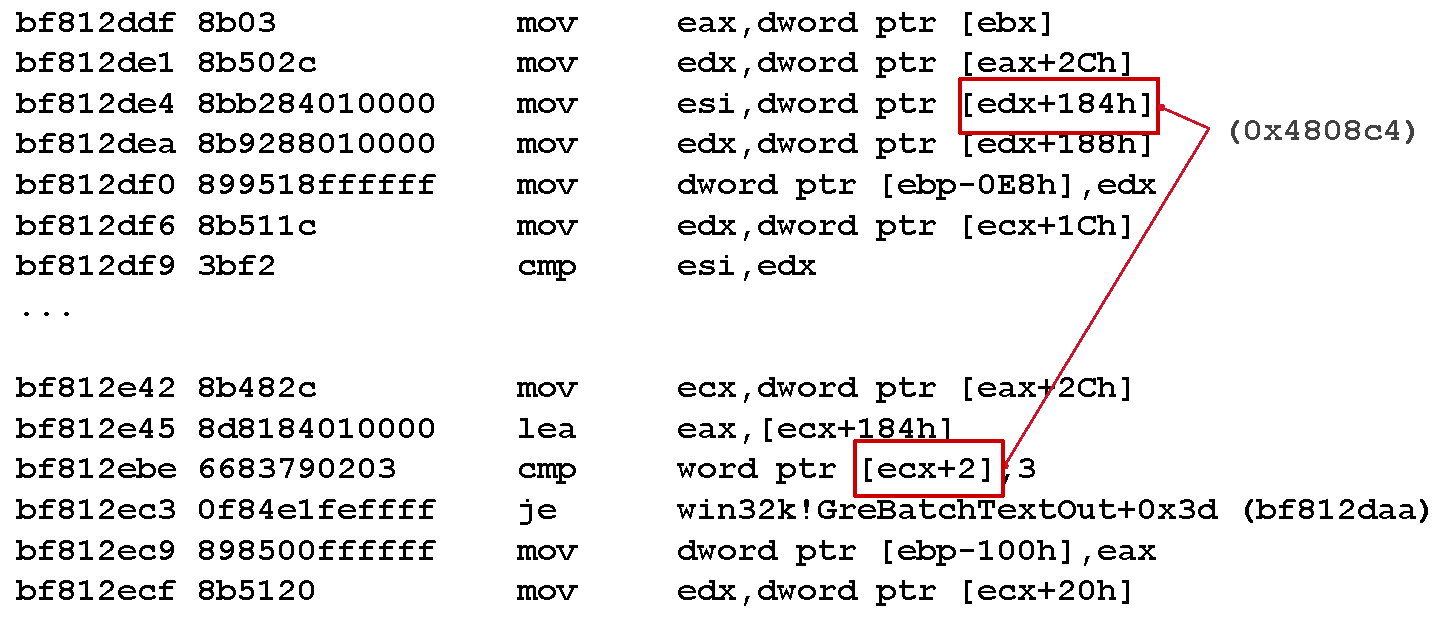
\includegraphics[width=0.47\textwidth]{figures/doublefetch}
  \centering
  \caption{CR3 0x6d40320; TEB 0x7ffdd000; EIP 0xbf812de4 and 0xbf812e4b read the same user-mode address 0x4808c4 within one system call.}
  \label{fig:doublefetch}
\end{figure}


Whether or not those bugs can further turn into vulnerabilities are case by case. However, a significant potential of those accesses is direct without a try-catch block. It may lead to a local denial-of-service (DOS) attack if the attacker can free the user-mode page right in front of the access. 
